\documentclass[a4paper,10pt]{report}
\usepackage[cm]{fullpage}
\usepackage[utf8]{inputenc}
\usepackage{amsmath}
\usepackage{amsthm}
\usepackage{amssymb}
\usepackage{booktabs}
\usepackage[table]{xcolor}
\usepackage{amssymb}
\usepackage{multirow}
\usepackage{fullpage}
\usepackage{float}
\usepackage{subfig}
\usepackage{graphicx}
\usepackage{listings}
\usepackage{color}
\usepackage{textcomp}

\usepackage{hyperref}

\definecolor{listinggray}{gray}{0.9}
%\definecolor{lbcolor}{rgb}{0.9,0.9,0.9}

\addtolength{\voffset}{-10pt}

\hypersetup{colorlinks=false}
 
\lstset{
%	backgroundcolor=\color{lbcolor},
	tabsize=4,
%	rulecolor=,
	language=python,
        basicstyle=\scriptsize,
        upquote=true,
        aboveskip={1.5\baselineskip},
        columns=fixed,
        showstringspaces=false,
        extendedchars=true,
        breaklines=true,
        prebreak = \raisebox{0ex}[0ex][0ex]{\ensuremath{\hookleftarrow}},
%        frame=single,
        showtabs=false,
        showspaces=false,
        showstringspaces=false,
        identifierstyle=\ttfamily,
        keywordstyle=\color[rgb]{0,0,1},
        commentstyle=\color[rgb]{0.133,0.545,0.133},
        stringstyle=\color[rgb]{0.627,0.126,0.941},
} \hypersetup{colorlinks=false}

\renewcommand\chaptername{Esperimento}
 
\DeclareGraphicsExtensions{.pdf,.png,.jpg}
 
\author{awa}
% Title Page
\title{Esperimento}

\begin{document}
\maketitle
\setcounter{tocdepth}{3}
\tableofcontents


\chapter{Viscosità}

\subsection{Da fare}
\begin{itemize}
 \item Grafici con barrette di errore
\end{itemize}

\section{Preambolo}
\subsection{Obiettivo di ricerca}
\subsection{Strumenti di laboratorio}

\section{Misurazioni preliminari}
\subsection{Sferette}
Abbiamo raccolto le seguenti misurazioni per quanto riguarda il diametro delle sferette:
\begin{center}
\begin{tabular}{|l|l|}
\toprule
 Sferette tipo 1: & 3mm\\
 Sferette tipo 2: & 4mm\\
 Sferette tipo 3: & 5mm\\
 Sferette tipo 4: & 6mm\\
\bottomrule
\end{tabular}
\end{center}

La sensibilità del calibro è di 0.05mm.\\
Peso delle sferette:

\begin{center}
\begin{tabular}{lll}
 Sferette tipo 1:
 & 0.1102g & 0.1102g \\
 & 0.1101g & \\
 \midrule
 Sferette tipo 2: 
 & 0.2612g & 0.2613g \\
 & 0.2613g & 0.2612g \\
 \midrule
 Sferette tipo 3: 
 & 0,5098g & 0,5100g \\
 & 0,5094g & 0,5100g \\
 & 0,5096g & 0,5098g \\
 \midrule
 Sferette tipo 4:
  & (3,521g/4) & 0.8806g \\
  & 0.8802g & 0.8807g \\
\end{tabular}
\end{center}

La sensibilità della bilancia è di $10^{-6}$ kg

In particolare, per una sferetta singola da 5mm, abbiamo ottenuto le seguenti misurazioni\\
\begin{tabular}{ccccccc}
0,5096g & 0,5098g & 0.5099g & 0,5095g & 0,5095g & 0,5096g & 0,5097g
\end{tabular}
\\
Per quanto riguarda il cilindro di glicerina, abbiamo segnato due tacche a una distanza di 15,1mm l'una dall'altra.
Per misurare questa distanza abbiamo utilizzato un metro a nastro con una sensibilità di 1mm.

\subsection{Dati sperimentali}
Di seguito le tabelle che registrano il tempo impiegato per attraversare il fluido.
\subsubsection{Sferette da 6mm}
\begin{tabular}{|c|c|c|c|c|c|c|c|c|c|}
\toprule
 1,68s & 1,68s & 1,65s & 2,21s* & 1,68s & 1,68s & 1,62s & 1,71s & 1,71s & 1,75s \\
 1,78s & 1,71s & 1,71s & 1,65s & 1,59s  & 1,65s  & 1,71s  & 1,68s & 1,68s & 1,65s \\
\midrule
 1,62s & 1,56s & 1,71s & 1,71s & 1,68s & 1,62s & 1,59s & 1,59s & 1,53s & 1,59s \\
 1,46s & 1,62s & 1,59s & 1,56s & 1,62s & 1,56s & 1,62s & 1,43s & 1,53s & 1,59s \\
\midrule
 1,56s & 1,56s & 1,53s & 1,62s & 1,68s & 1,56s & 1,56s & 1,59s & 1,59s & 1,50s\\
 1,53s & 1,62s & 1,50s & 1,56s & 1,59s & 1,62s & 1,43s & 1,62s & 1,43s & 1,40s \\
\midrule
 1,59s & 1,46s & 1,46s & 1,59s & 1,65s & 1,59s & 1,68s & 1,43s & 1,53s & 1,62s \\
 1,46s & 1,50s & 1,56s & 1,59s & 1,50s & 1,59s  & 1,59s & 1,59s & 1,53s & 1,59s \\
\midrule
1,59s & 1,46s & 1,53s & 1,43s & 1,53s & 1,46s & 1,46 & 1,56 & 1,40s & 1,34s \\
1,46s & 1,37s  & 1,50s   & 1,50s  & 1,43s & 1,31s & 1,40s  & 1,43s  & 1,34s & 1,43s \\
\bottomrule
\end{tabular}
\subsubsection{Sferette da 5mm}
\begin{tabular}{|c|c|c|c|c|c|c|c|c|c|}
\toprule
 2,34s* & 2,43s* & 2,31s & 2,21s & 2,12s & 2,53s* & 2,21s & 2,21s & 2,71s* & 2,71s* \\
 2,12s & 2,34s & 2,18s & 2,34* & 2,12s & 2,06s & 2,12s & 2,59s* & 2,03s & 2,06s \\
\midrule
 2,87s* & 2,21s & 2,21s & 2,12s & 2,03s & 2,09s & 2,12s & 2,46* & 2,06s & 2,25s \\
 2,15s & 2,25s & 2,00s &  &  &  &  &  &  & \\
\bottomrule
\end{tabular}
\subsubsection{Sferette da 4mm}
\begin{tabular}{|c|c|c|c|c|c|c|c|c|c|}
\toprule
 3,06s & 3,09s & 3,15s & 3,12s & 3,03s & 3,15s & 3,25s & 3,25s & 3,18s & 3,09s \\
 3,09s & 3,09s & 3,21s & 3,12s & 3,06s & 3,06s & 3,15s & 3,46s & 3,25s & 3,12s \\
\bottomrule
\end{tabular}
\subsubsection{Sferette da 3mm}

\begin{tabular}{|c|c|c|c|c|c|c|c|c|c|}
\toprule
 5,28s & 5,09s & 4,96s & 5,25s & 5,28s & 5,12s & 5,06s & 5,12s & 5,06s & 5,28s \\
 5,03s & 5,06s & 4,87s & 4,90s & 4,96s & 5,06s & 5,06s & 4,95s & 4,93s & 5,18s \\
 5,18s & 5,18s & 5,21s & 4,87 & 5,34s &  &  &  &  & \\
\bottomrule
\end{tabular}

* = per queste misurazioni, la pallina si è avvicinata molto alla parete del tubo, e dunque le misurazioni potrebbero essere falsate.
TODO: rimuovi i vecchi valori

\section{Elaborazione dei dati}
\subsection{Calcolo dei tempi}
Per le sferette da 6mm abbiamo scartato il valore 2,21s, connotato dall'asterisco, in quanto evidente errore sperimentale. A conferma di ciò, si trova che esso esso dista circa 6,5 deviazioni standard dal valore medio.

[tabelle statistiche]
- Gaussiane+istogrammi
- Plotting dei dati
- Tabelle di conti (frequenze assolute, relative, ...)

\subsubsection{Note operative}
Abbiamo eliminato alcuni dati

\subsection{Estrapolazione}
- Grafici velocità (lin, quad e log)
- Calcolo di astar, bstar

\subsection{Sezione teorica}
Abbiamo usato le seguenti formule statistiche per....

\subsection{Conclusioni}

\chapter{Pendolo a torsione}
\section{Introduzione}
\subsection{Oggetto della ricerca}
L'esperienza si prefissa l'obiettivo di misura le costanti di torsione $c$ di tre fili di sezione differente. 
\subsection{Metodo}
L'esperienza si compone di tre differenti fasi.
\begin{itemize}
\item Misura sperimentale dello spostamento angolare a seguito del momento della forza peso, al fine di calcolarne il momento d'inerzia 
\item Misura sperimentale del periodo di un pendolo di torsione, al fine di calcolare la costante di torsione dei fili
\item Misura della costante $c$ di torsione tramite l'instaurazione di un equilibrio tra il momento elastico e il momento della forza peso, e confronto con il valore teorico di $c$
\end{itemize}
\subsection{ Strumentazione e dati geometrici}
Nell'esperimento verrà utilizzato un pendolo di torsione strutturato nel seguente modo:
\\
Micrometro: $ \pm 1 \mu m$
 \\
Metro: $\pm 1 mm$
\\
Sensore di rotazione: $\pm 0.09$ gradi
\\

\begin{tabular}{ll}
Masse puntiformi: & 0.074 kg\\
Lunghezza sbarra: & 0.38 m\\
Massa Sbarra: & 0.2563 kg\\
Raggio Sbarra: & 0.0045 m\\
\midrule
Massa anello: & 0.46927 kg\\
Raggio interno: & 0.0265 m\\
Raggio esterno: & 0.0355 m\\
\midrule
Supporto & 0.0035 m\\
\midrule
Massa disco: & 0.12055 kg\\
Raggio disco: & 0.0475 m\\
Diametro carrucola: & 29 mm\\
\end{tabular}

\section{Raccolta dei dati}
Per quanto riguarda i tre fili in esame:
\begin{center}

\begin{tabular}{l|l|l|l}
 & Filo A & Filo B & Filo C \\
\midrule
Diametro (mm) & 1.750 & 1.175 & 0.880 \\

Lunghezza (cm) & 41.3 &  43 & 33.5 \\
\midrule
\end{tabular}\end{center}

\subsection{Misura dei momenti d'inerzia}

In questa fase si provvederà a ricavare  sperimentalmente i momenti d'inerzia dei seguenti corpi:
\begin{itemize}
\item Disco 
\item Anello
\item Sbarra cilindrica omogenea, con due masse uguali, scorrevoli su di essa, poste equidistanti dall’asse di rotazione (a una distanza \textbf{VEDI QUADERNO}
\end{itemize}

Si è utilizzato un sistema di due pulleggie e un sensore di rotazione.
Il sensore di rotazione fornisce la posizione angolare in funzione del tempo. 



- Grafico angolo/tempo cadute?
- Grafico accelerazione/tempo cadute?
\\
\begin{center}
\begin{tabular}{c|ccc}
Oggetto & Accelerazione lineare & Accelerazione angolare & Momento d'inerzia \\
\midrule
Disco & \\
Anello & \\
Sbarra &\\
\end{tabular}
\end{center}
Acquisiti i dati della posizione angolare in funzione del tempo, è possibile calcolare l'accelerazione angolare del sistema. A questo punto, si può calcolare $I$ nel seguente modo:
$$ bF_p = I\alpha $$
La forza peso ($F_p$) è nota, così come il braccio ($b$) e, dall'elaborazione dei dati sperimentali, possiamo calcolare $\alpha$.

seguenti corpi, elencati con i rispettivi momenti d'inerzia \textbf{teorici}:
$$ I_{sbarra} = \frac{1}{2} m R^2 = 0.00844 $$
$$ I_{anello}?? =\frac{1}{2} m (R^2_1 + R^2_2) = 0.00046 $$
$$ I_{disco}?? = \frac{1}{12} m L^2 + 2 \mu D^2 = 0.00013 $$



\subsection{Pendolo di torsione}

Abbiamo ricavato i seguenti periodi di oscillazione per ogni filo:
\\
\begin{tabular}{cc}
\includegraphics[scale=0.4]{../grafici/FiloA.png}
&
\includegraphics[scale=0.4]{../grafici/FiloB.png}
\\
\begin{tabular}{ll}
Filo A: & $0.644 \pm 0.015\ s$\\
Filo B: & $2.429 \pm 0.033\ s$\\
Filo C: & $3.844 \pm 0.046\ s$
\end{tabular}
&
\includegraphics[scale=0.4]{../grafici/FiloC.png}

\end{tabular}


Questo ci permette di calcolare la costante di torsione $c$ sfruttando la seguente eguaglianza:
$$ -c\theta = I\frac{d^2\theta}{d\theta^2} $$
che identifica un moto oscillatorio di periodo
$$ T = 2\pi \sqrt{\frac{I}{c}}$$
da cui
$$ c = 4\pi^2\frac{I}{T^2} $$

\begin{tabular}{l|l l}
& Periodo (s) & Costante di torsione () \\
\midrule
Filo A & \\
Filo B & \\
Filo C & \\
\end{tabular}


\subsection{Misura di equilibrio}

Tabulati gli angoli di deflessione per ogni filo in base alla massa sospesa (controlla!)\\
\begin{center}
\begin{tabular}{l|lll}
& A & B & C \\
\midrule
50g & 4.0 & 12.0 & 31.0 \\
100g & 7.0 & 23.0 & 61.0 \\
200g & 13.0 & 47.0 & 126.0 \\
\midrule
\end{tabular}\end{center}
Essendo il pendolo in equilibrio, poniamo
$$ \tau_{peso} = b\cdot mg = c\theta $$
da cui
$$ c = \frac{b\cdot mg}{\theta} $$
dove $b$ è il braccio di applicazione della forza peso, ovvero il raggio della carrucola.
I valori di $c$ calcolati sono dunque stati (in $N\cdot m/rad$):

\begin{center}
\begin{tabular}{l|lll}
Peso & Filo A & Filo B & Filo C \\
\midrule
50g & 0.1019 & 0.0340 & 0.0135 \\
100g & 0.1164 & 0.0354 & 0.0134 \\
200g & 0.1254 & 0.0347 & 0.0129 \\
\midrule
$c_{best}$ & $0.115$ & $0.035$& $0.013$ \\
$\sigma_{c}$ & $0.012$ & $\sim0$ & $\sim 0$ \\
\end{tabular}
\end{center}

\section{Dipendenza di $c$ da $r^4$}

Per la misura statica di $c$, bisogna utilizzare la seguente relazione:

$$ c = G \frac{\pi}{2}\frac{r^4}{l} $$

dove $G$ è il modulo di rigidità o di scorrimento ed è una proprietà specifica del materiale di cui il filo è realizzato.

Non siamo riusciti a trovare i valori di G tabulati in quanto non conoscevamo il materiale in cui era costruito il filo, quindi abbiamo cercato di arrivare a una migliore stima per riconoscerlo. Abbiamo utilizzato il valore di $c$ misurato in precedenza (misura statica) per calcolare $G$ secondo la seguente formula:

$$ G = \frac{2cl}{\pi r^4} $$

I valori calcolati sono stati:
\begin{center}
\begin{tabular}{lll}
Filo A & Filo B & Filo C \\
\midrule
49 GPa & 78 GPa & 73 GPa \\
\end{tabular}
\end{center}

Da cui abbiamo supposto che il filo A fosse in acciaio, e i fili B e C in titanio.
I dati ufficiali tabulati infatti sono i seguenti:
\begin{center}
\begin{tabular}{ll}
Acciaio & Titanio \\
\midrule
41 GPa & 78 GPa \\
\end{tabular}
\end{center}
Ripetendo il calcolo con G come tabulato, otteniamo:
\begin{center}
\begin{tabular}{lll}
Filo A & Filo B & Filo C \\
\midrule
0.0914 & 0.0339 & 0.0137 \\
\end{tabular}
\end{center}
\section{Conclusioni}
Confrontiamo i valori di $c$ teorici e calcolati tramite il metodo statico:
\begin{center}
\begin{tabular}{l|lll}
& Filo A & Filo B & Filo C \\
\midrule
Misura statica & $0.115$ & $0.035$& $0.013$ \\
Misura teorica & 0.0914 & 0.0339 & 0.0137 \\
\midrule
Misura media & \\
Errore ($\frac{\Delta c}{\bar{c}}$) & \\
\end{tabular}
\end{center}



\chapter{Oscillazioni smorzate e forzate}


\section{Introduzione}
\subsection{Oggetto della ricerca}
L'oggetto di questa ricerca è lo studio delle oscillazioni smorzate e forzate di un pendolo. Studiando il variare delle oscillazioni con il variare della frequenza operativa della forzante, si studierà il fenomeno della risonanza.

\subsection{Strumenti}
\begin{center}
\begin{tabular}{l|l}
\midrule
Strumento & Precisione\\
\midrule
Calibro & $\pm 0.05$ mm\\ 
Sensore di rotazione & $\pm 0.00157$ rad\\ 
Alimentatore & $\pm 0.01$ V\\ 
\midrule 
\end{tabular}
\end{center}
L'attrezzatura utilizza è costituita da un disco metallico attaccato ad una puleggia. La puleggia è messa in oscillazione da un filo alle cui estremità vi sono un oscillatore  elettromeccanico e un sistema di due molle. Al disco è possibile avvicinare e allontanare un magnete, fissato su una vite. 

\subsection{Metodo in breve}
L'esperimento è suddiviso in tre fasi:

\begin{itemize}
\item \textbf{Oscillazioni pseudo-libere}
Si ponga in oscillazione il disco, con il magnete  posizionato lontano e l'oscillatore elettromeccanico spento. Si misuri il periodo delle oscillazioni libere.
\item \textbf{Oscillazioni smorzate}
Si avvicini il magnete al disco metallico. Il moto oscillatorio risulterà così smorzato per effetto delle correnti di Focault 
\item \textbf{Oscillazioni smorzate e forzate}
Per queste misurazioni, si metta in azione l'oscillatore elettromeccanico, che fornisce una componente forzante. Variando il voltaggio dell'alimentatore,  la frequenza di rotazione dell'oscillatore cambia. Si cerchi la frequenza di risonanza del sistema.
\end{itemize}

[se la consegnamo, aggiungi diagramma]

\section{Raccolta dati}

I seguenti grafici rappresentano la posizione in funzione del tempo delle oscillazioni in esame. Sono state rilevate da un sensore di moto rotatorio, collegato al disco metallico. 
Nella sezione "oscillazioni smorzate-forzate", ci siamo serviti di una fotocellula per misurare il periodo della forzante generata dall'oscillatore elettromeccanico. 

\subsection{Oscillazioni libere}

- Grafici posizione tempo 

\subsection{Oscillazioni smorzate}

- Grafici 
\subsection{Oscillazioni smorzate-forzate}

- Grafici

\section{Analisi dati}

\subsection{Oscillazioni libere}
In questa prima fase dell'analisi dei dati, estrapoliamo dalla posizione in funzione del tempo, il periodo dell'oscillazione libera. Essendo un sistema reale, risultata comunque smorzato dalla presenza di attriti. 


\subsection{Oscillazioni smorzate}

Abbiamo ricavato i valori dei parametri liberi utilizzando il programma DataStudio, e interpolando i dati con la seguente equazione:
$$ \theta (t) = A_0 e^{- \gamma t} \sin(wt+\phi)+\theta_0 $$


Dunque, noti $\omega$ e $\gamma$, è possibile calcolare $ \omega_0 $, cioè la pulsazione per le oscillazioni libere, tramite l'equazione:
$$ \omega = \sqrt{\omega_0^2 - \gamma^2} $$

e confrontarlo con il valore che avevamo ricavato interpolando direttamente il grafico delle oscillazioni libere

$$\omega_0 = 4.272\ rad/s$$

\subsubsection{4.80mm}

\begin{center}
\begin{tabular}{l|l|l}
\midrule
Parametri & Valore ricavato & $ \pm \sigma$ \\
\midrule
$A_0$ & 3.08 rad & 0.020\\
$\gamma$ & 0.197 $m^4/kg$& 0.0019\\
$\omega$ & -4.27 rad/s& 0.0019\\
$\phi$ & 1.93 rad & 0.0069 \\
$\theta_0$ & -1.53 rad& 0.0019 \\
\midrule
\end{tabular}
\end{center}

Il valore così calcolato è leggermente maggiore di quello ricavato dalla misurazione diretta. $$\omega_{0} = 4.275\ rad/s$$

Questo risultato è in perfetto accordo nei limiti della precisione dello strumento.
\subsubsection{2.80mm}

\begin{center}
\begin{tabular}{l|l|l}
\midrule
Parametri & Valore ricavato & $ \pm \sigma$ \\
\midrule
$A_0$ & 3.40 rad & 0.020\\
$\gamma$ & 0.636 $m^4/kg$& 0.0057\\
$\omega$ & -4.25 $rad/s$& 0.0064\\
$\phi$ & 2.38 $rad$ & 0.0076 \\
$\theta_0$ & -0.57 $rad$& 0.0038 \\
\midrule
\end{tabular}
\end{center}

$$\omega_{0} = 4.297\ rad/s$$

\subsubsection{1.00mm}

\begin{center}
\begin{tabular}{l|l|l}
\midrule
Parametri & Valore ricavato & $ \pm \sigma$ \\
\midrule
$A_0$ & 18600 rad & 1300 \\
$\gamma$ & 1.50 $m^4/kg$& 0.0011\\
$\omega$ & 4.02 rad/s& 0.0077\\
$\phi$ & 26.3 rad & 0.0046 \\
$\theta_0$ & 0.055 rad& 0.0016 \\
\midrule
\end{tabular}
\end{center}

$$\omega_{0} = 4.291\ rad/s $$

\subsection{Oscillazioni smorzate-forzate}
Tramite l'interpolazione dei grafici di posizione angolare in funzione del tempo con una funzione\\
sinosuidale, sono stati trovati i valori dell'ampiezza e del periodo di ognuna delle oscillazioni.

Dopodiché abbiamo interpolato questi dati con il programma DataStudio, secondo la funzione
$$ A(\omega) = \frac{M_0}{\sqrt{ ({\omega_0}^2-\omega^2)^2 + 4\gamma^2\omega^2}} $$

e lasciando liberi i parametri $M_0$, $\gamma$ e $\omega_0$ abbiamo trovato alcuni valori. Abbiamo omesso di trascrivere gli errori quando questi erano palesemente trascurabili.

\clearpage

\subsubsection{4.80mm}
\begin{center}

\includegraphics[scale=0.75]{"../grafici/Magnetea48mm"}
\end{center}
\begin{center}
\begin{tabular}{l|l|l}
$\omega$ (rad/s) & Periodo (s) & A (rad) \\
\midrule
1.15	& 5.45 & 0.89\\
1.31	& 4.78 & 0.94\\
1.75	& 3.57 & 1.05\\
1.97	& 3.19 & 1.09\\
2.42	& 2.59 & 1.30\\
2.55	& 2.46 & 1.30\\
3.05    & 2.06 & 1.84\\
3.31	& 1.90 & 1.91\\
3.69	& 1.70 & 3.42\\
3.95	& 1.59 & 6.35\\
4.94	& 1.27 & 2.48\\
5.19	& 1.21 & 1.74\\
5.51	& 1.14 & 1.19 \\
\midrule

\end{tabular}
$$ \omega_0 = 4.25\ rad/s $$
$$ \gamma = 0.193\ s^{-1}$$
$$ M_0 = 15.3\ s$$


\end{center}




\subsubsection{2.80mm}
\begin{center}
\begin{tabular}{l|l|l}
$\omega$ (rad/s) & Periodo (s) & A (rad) \\
\midrule
3.14 & 2.00 & 1.68 \\
3.85 & 1.63 & 2.95 \\
4.36 & 1.44 & 3.22 \\
4.83 & 1.30 & 2.17 \\
5.06 & 1.24 & 1.67 \\
5.46 & 1.15 & 1.20 \\
5.71 & 1.10 & 0.99 \\
6.40 & 0.98 & 0.68 \\
7.06 & 0.89 & 0.51 \\
8.49 & 0.74 & 0.26 \\
\midrule
\end{tabular}
\end{center}
\includegraphics[scale=0.75]{"../grafici/Magnetea28mm"}



$$ \omega_0 = 4.26\ rad/s $$
$$ \gamma = 0.543\ s^{-1} $$
$$ M_0 = 15.6\ s$$


\subsubsection{1.00mm}
\begin{center}
\begin{tabular}{l|l|l}
$\omega$ (rad/s) & Periodo (s) & A (rad) \\
\midrule
3.12 & 2.01 & 1.33 \\
3.39 & 1.85 & 1.42 \\
3.76 & 1.67 & 1.45 \\
4.07 & 1.54 & 1.47 \\
4.52 & 1.39 & 1.31 \\
4.79 & 1.31 & 1.18 \\
5.15 & 1.22 & 1.01 \\
5.28 & 1.19 & 0.88 \\
5.76 & 1.09 & 0.76 \\
6.10 & 1.03 & 0.65 \\
6.75 & 0.93 & 0.49 \\
7.39 & 0.85 & 0.39 \\
\midrule
\end{tabular}
\end{center}
\includegraphics[scale=0.75]{"../grafici/Magnetea10mm"}


$$ \omega_0 = 4.37\ rad/s $$
$$ \gamma = 1.40 \pm 0.14\ s^{-1}$$
$$ M_0 = 17.1 \pm 1.4\ s$$

Spiegazione fenomeno risonanza

% 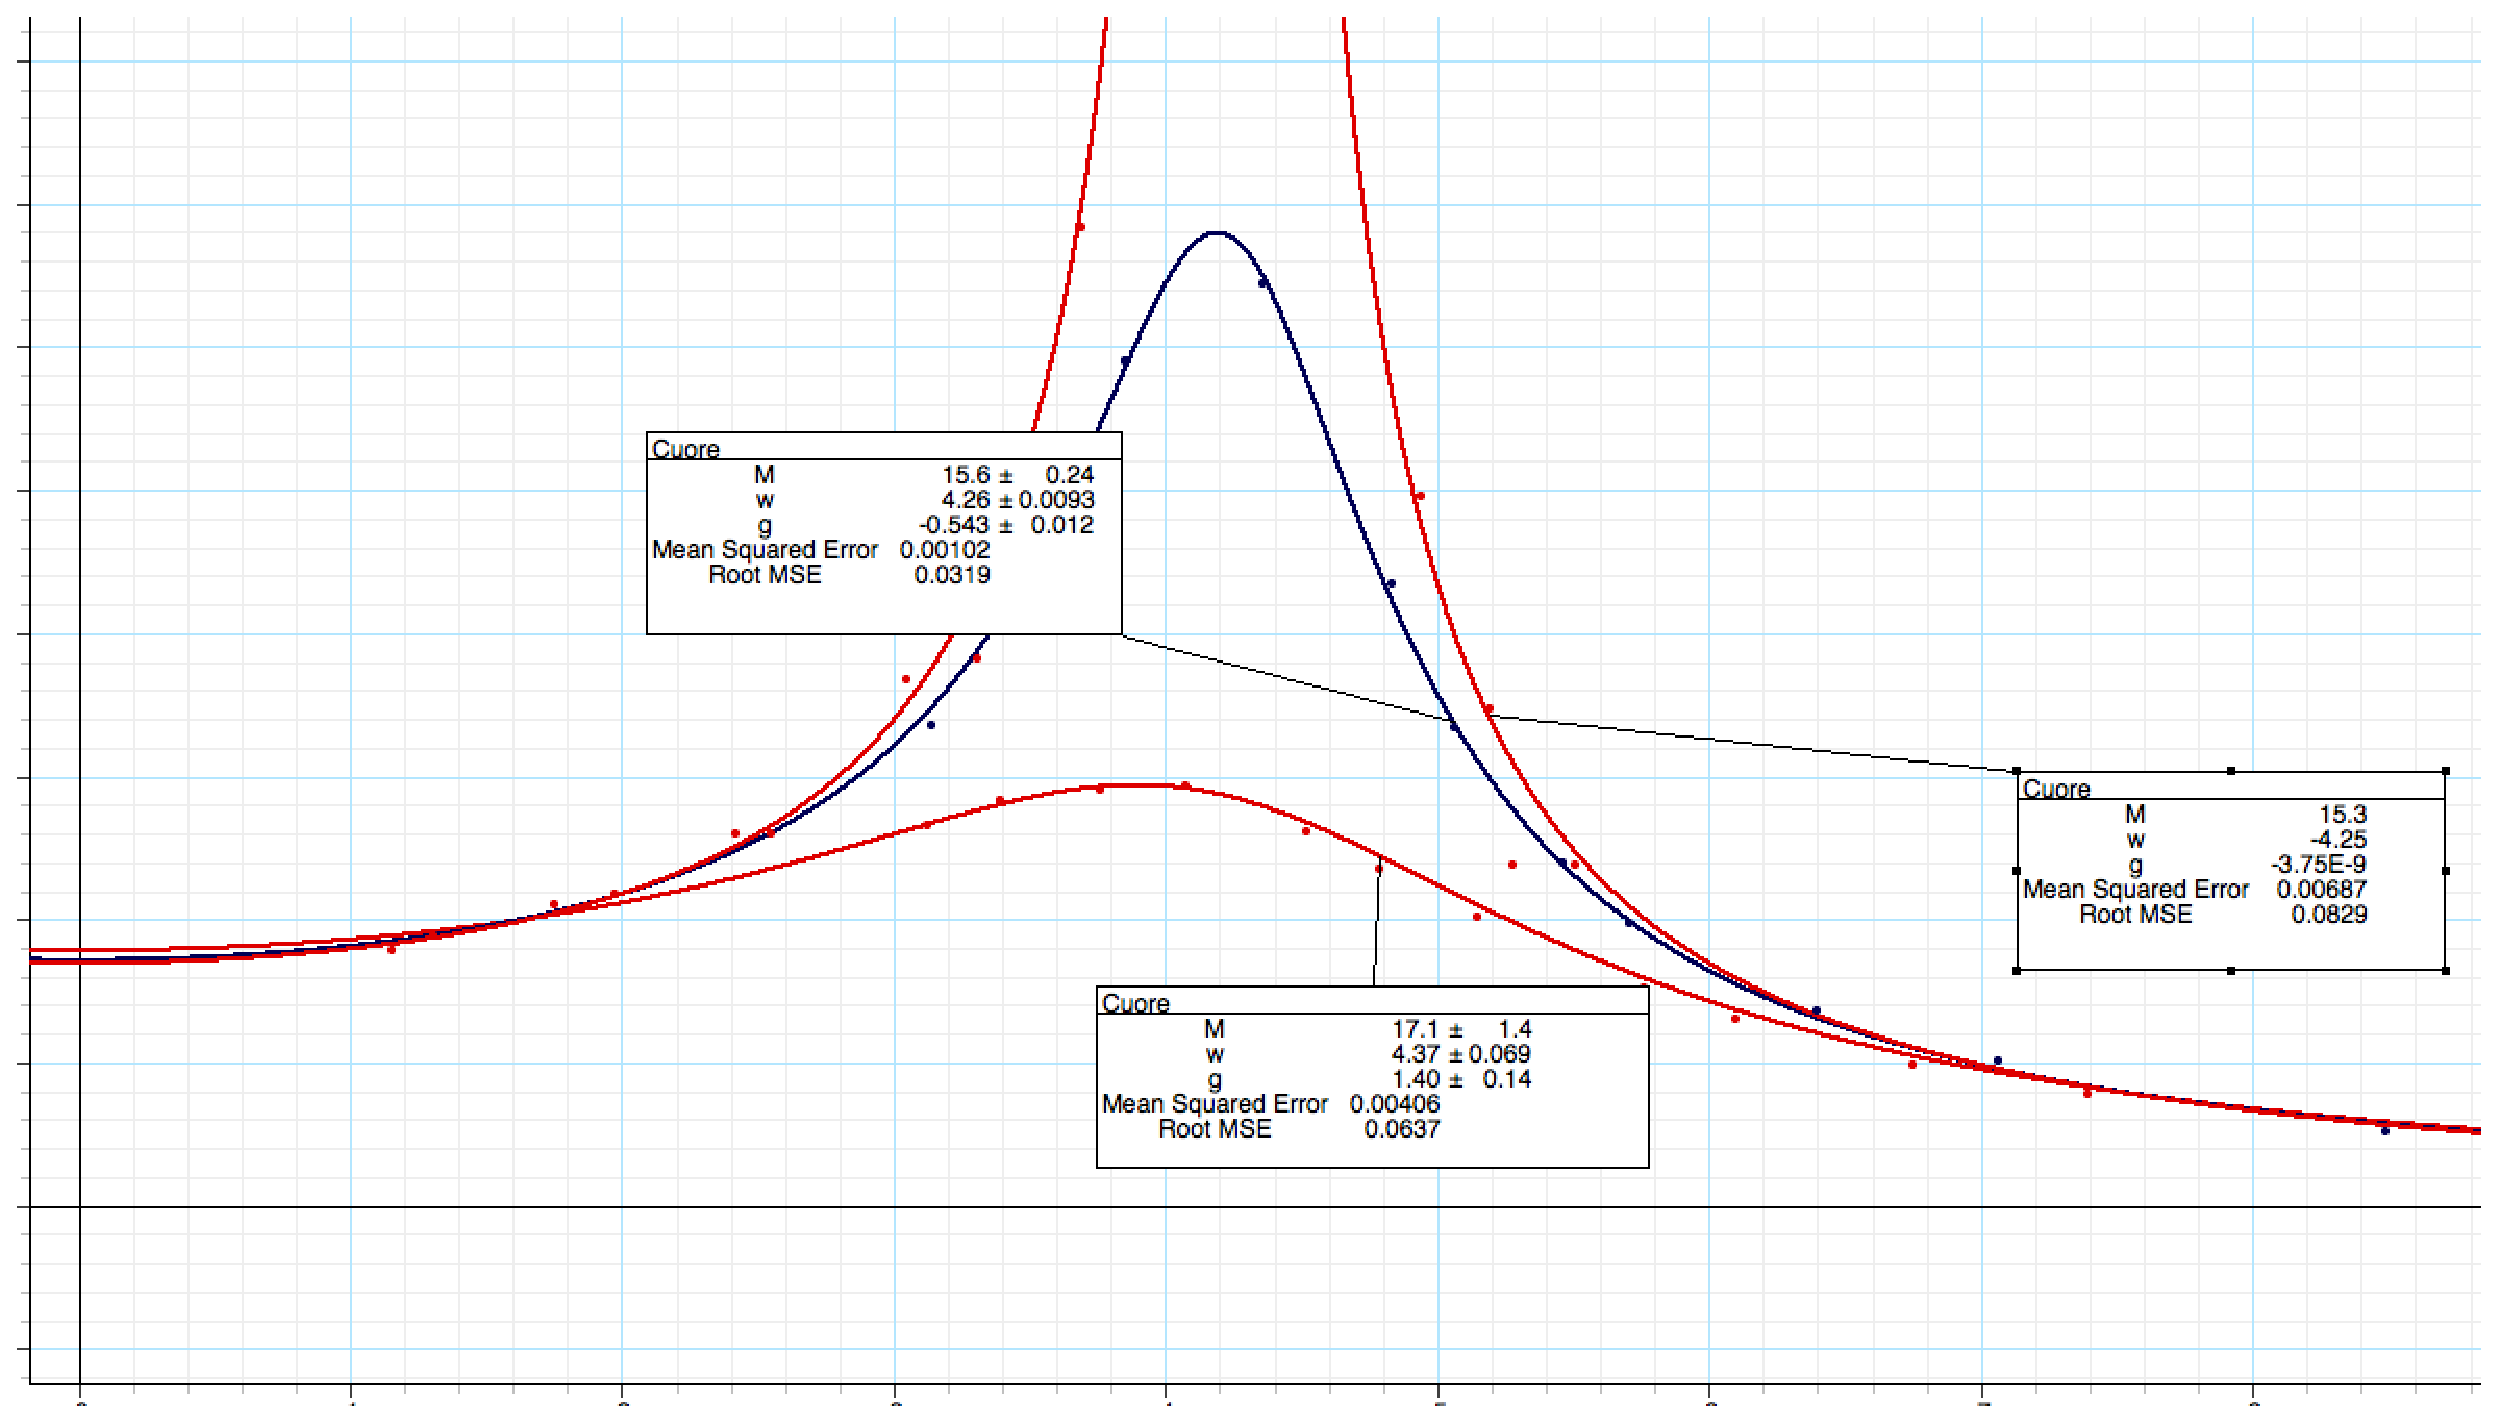
\includegraphics[scale=0.2]{graf}
%Fare grafico tutti insieme?

\section{Conclusioni}
L'esperimento è riuscito un sacco.

\section{Fenomeno}
Sovvrapponendo le curve trovate in precedenza, possiamo apprezzare un grafico nel quale si mette in evidenza la risonanza. 
Verifichiamo anche la condizione di risonanza Con l'approssimarsi di $\gamma $ a zero, il valore dell'ampiezza tende a $\infty$.




























































\includegraphics[scale=0.9]{../grafici/risonanza}

\chapter{Bilancia di Cavendish}
\section{Introduzione}
\subsection{Oggetto della ricerca}
Misurazione della costante di gravitazione G mediante la bilancia di Cavendish.
\subsection{Proprietà geometriche dei corpi e strumentazione}

\begin{tabular}{ll}
m=38.3$\pm$0.2 g & massa sfere piccole\\
M=1500$\pm$10 g	 & massa sfere grandi\\
r=9.53 mm & raggio sfere piccole\\
R=31.9 mm	 & raggio sfere grandi\\
$m_c\cong 2m$ & massa manubrio\\
\end{tabular}
\\
Il momento d'inerzia $I$ del corpo si calcola:

$$ I=2m(d^2+2/5r^2)$$
L'inerzia del corpo è:
$I = 1.94283 \cdot 10^{-4} kg\cdot m^2$
L'incertezza sul momento di inerzia è nell'ordine di $10^{-6}$, perciò è trascurabile. 
\subsection{Metodo in breve}



\section{Misura $k$ e $\theta$}
L'incertezza relativa allo strumento per la misurazione del periodo è trascurabile rispetto l'entità della misura. 
Il periodo misurato è:

$$T^2 = 4 \pi^2 \frac{I}{k}$$
Quindi
$$k = 4 \pi^2 \frac{I}{T^2}$$

$$k = 2.84 \cdot 10^{-8} kg \cdot \frac{m^2}{s^2}$$

Per trovare la posizione di equilibrio, $S_1$ utilizziamo la formula ricorsiva:

$$X_m = \frac{\frac{X_1+X_3}{2} +X_2}{2}$$ 

\begin{tabular}{c|*{7}{c}}
$2k\pi$ & \\
\midrule
$(2k+1)\pi$ & \\
\end{tabular}

$$G = -\frac{k \theta b^2}{2mMd} $$

\section{Analisi dati} 

\section{Conclusioni}


\chapter{Banco Ottico}
\section{Introduzione}
\subsection{Scopo dell'esperimento e metodo in breve}

L'esperimento si compone di tre parti. Nella prima, si verifica la validità della Legge di Snell e la reversibilità del cammino ottico: dato un raggio luminoso attraversante un semi-cilindro in plexiglass, misuriamo l'angolo di incidenza $\theta_{rifrazione}$ ed il corrispondente  angolo di rifrazione $\theta_{rifrazione}$. Sempre grazie alla legge di Snell si ricerca la miglior stima dell'indice di rifrazione del plexiglass $n$.
\\


Nella seconda parte, si ricerca $n$ studiando l'angolo di deviazione minima $\delta_{min}$ di un prisma a base triangolare e di un prisma a base trapezoidale. Inoltre, si ricerca la distanza di cui viene traslato il raggio, che arriva con un certo angolo di incidenza $\theta$, quando passa per due superfici parallele.
\\

Infine si verifica la legge dei punti coniugati tramite la misura delle distanze $p$ e $q$ e la validità dell'ingrandimento ottico $M$. 

\subsection{Strumenti}
In questa tabella vengono riassunti gli strumenti rivelatori utilizzati, con le relative precisioni, e il set-up dell'esperimento.
\begin{center}
\begin{tabular}{c|c}
Strumento & Precisione \\
\midrule
Piatt. Graduata & $\pm 1 grado $ \\
Metro & $\pm 1 mm $\\
\end{tabular}
\end{center}

Per le prime due parti dell' esperimento, il proiettore è stato impostato sulla modalità a singolo raggio luminoso e successivamente sulla modalità oggetto per la terza e ultima parte. 
Il proiettore, insieme alla piattaforma girevole graduata, alle lenti ed a uno schermo bianco, può scorrere liberamente lungo una rotaia, permettendo di modificare le distanze tra gli oggetti a piacimento.

\section{Reversibilità del cammino luminoso}

Tutte le misure seguenti sono espresse in gradi.


\begin{table}
\center
\begin{tabular}{c|c||c|c}
 \multicolumn{2}{c}{\textit{Faccia piana}} &
\multicolumn{2}{c}{\textit{Faccia curva}} \\
$\theta_{incidenza} $ & $\theta_{rifrazione} $ &$\theta_{incidenza} $ & $\theta_{rifrazione} $\\
\midrule
 10 & 7 & 7 & 10 \\
15 & 10 & &\\
20 & \textbf{13.5} & 13.5 & 20\\ 
25 & \textbf{16.5} & & \\
30 & 20 & 30 & 20\\
40 & 26 & 26 & 40\\
35 & 23 & &\\
45&  \textbf{28.5} & & \\
\end{tabular}
\caption*{Misure in gradi}
\end{table}


Raccolti i valori degli angoli di incidenza e dei corrispondenti angoli di rifrazione, possiamo calcolare la miglior stima di $n$.
La legge di Snell esprime la relazione che lega gli indici di rifrazione dei due materiali attraversati dal raggio luminoso, e i seni degli angoli di incidenza e rifrazione:

\begin{center}
$n_1 sin\theta_1 = n_2 sin\theta_2$
\end{center}

Poiché $n_a \simeq1 $ ( indice di rifrazione dell'aria ), si ricava:

$$n_2 = \frac{sin\theta_1}{sin\theta_2}$$

Nell'elaborazione dei dati, abbiamo selezionato solo le coppie di misure cui corrispondesse un errore relativo percentuale minore del 6\%, al fine di avere una stima più precisa del valore vero di $n$.

\begin{center}
\begin{tabular}{c|c|c|c|c|c}
\textbf{$\theta_1$} & 25 & 30 & 40 & 35 & 45\\
\midrule
\textbf{$\theta_2$} & 16.5 & 20 & 26 & 23 & 28.5\\
\midrule
\textbf{$n_i$} (*) & 1.489 & 1.462 & 1.468 & 1.468 & 1.482\\
\end{tabular}\\

\end{center}

(*) in questo caso abbiamo tenuto un numero superiore di cifre significative, in quanto si tratta di calcoli intermedi 
%Ripensare alle cifre significative

$$\overline{n} = \frac{\displaystyle\sum\limits_{i=1}^N n_i}{N} = 1.474 $$

$$\sigma_n = \sqrt{\frac{\sum_{i=1}^N n_i}{N-1}} = 0.01$$

$$\sigma_{\overline{n}} = \frac{\sigma_n}{\sqrt{N}} = 0.004$$

$$n_{best} = 1.474  \pm 0.004 $$

%Cifre significative incertezza diverse da cifre significative misura!

\section{Misura dell'angolo di deviazione minima}


L'angolo di deviazione minima ($\delta_{min}$) è il più piccolo angolo misurato facendo incidere un fascio di luce sulla faccia di un prisma (con inclinazione variabile) e misurando l'ampiezza dell'angolo rifratto. Nel nostro esperimento abbiamo utilizzato due prismi: uno con base un triangolo equilatero e l'altro un trapezio rettangolo.
\\

In tabella sono riportati i valori trovati per ogni misurazione dell'angolo rifratto. Per aumentare il livello di precisione, abbiamo raccolto i dati relativi agli angoli di deviazione minima per ogni faccia di prisma a base triangolare, identificando ogni misurazione con il numero dello spigolo compreso tra le facce colpite e il verso di percorrenza della luce.
\\

Per ovvie ragioni geometriche, nel caso del prisma a base trapezoidale (è presente un solo angolo acuto, di 45 gradi) è stato impossibile effettuare misure riferite a vari vertici.

\begin{center}
\begin{tabular}{|c | c | c|}
\hline
Spigolo & $\delta_{min}$ (andata) & $\delta_{min}$ (ritorno)\\
\hline
\multicolumn{3}{|c|}{\textit{Prisma a base triangolare}} \\
\hline
1 & 41 & 31\\
2 & 43 & 39\\
3 & 41 & 41\\
\hline
\multicolumn{3}{|c|}{\textit{Prisma a base trapezoidale}} \\
\hline
1 & 28 & 21\\
\hline
\end{tabular}
\end{center}

$$\overline{\delta}_{min} = \frac{\displaystyle\sum\limits_{i=1}^6 \delta_i}{6} = 1.52$$

%Angolo deviazione minima, immagine
\subsection{Analisi dei dati}

\section{Lenti sottili}
\
Nell'ultima parte dell'esperimento, si verifica la validità della legge dei punti coniugati,
$$ \frac{1}{f} = \frac{1}{q} + \frac{1}{p} $$
\textit{p: distanza sorgente-lente}
\textit{q: distanza lente-schermo}
\textit{d: diametro circonferenza proiettata}

In tabella sono riportati sulla destra le misure effettuate con lente di focale $f=100 mm$, a sinistra con lente di focale $f=200mm$. Tutti i valori sono in cm.

\begin{center}
\begin{tabular}{*{3}{c|}*{3}{|c}}
p & q &d &p &q&d\\
\midrule
13.5 & 36.5 & 5.5 & 73.4 & 26.6 & 0.7\\
36.2 & 13.8 & 0.8 & 26.4 & 73.6 & 5.5\\
\midrule
18.0 & 22.0 & 2.5 & 61.5 & 28.5 & 0.9\\
22.0 & 18.0 & 2.1 & 28.1 & 61.9 & 4.8\\
\end{tabular}
\end{center}

Per verificare la validità, rappresentare su un grafico i punti ($\frac{1}{p};\frac{1}{q})$ e verificare che i punti sono disposti lungo una retta. 
\\
\includegraphics[scale=0.75]{../grafici/ottica}

L'intecetta trovata è $q_1 = 0.1024$ e $q_2 = 0.05108$.
Ricaviamo i valore della focale $f = \frac{1}{q}$. $f_{1} = 9.76\  cm$ e $f_{2} = 19.57\ cm$. 

L'incertezza sulla focale è data dall'espressione:
$$\delta f = \sqrt{\frac{q^4(\delta p)^2 + p^4(\delta q)^2}{(p+q)^2}}$$

ottenuta tramite il metodo delle derivate parziali.

$$\delta f_{1} = \pm 2.66\ cm $$ 
$$ \delta f_{2} = \pm 5.43\ cm $$




\chapter{Pendolo di Kater e caduta libera}
\section{Introduzione}

L'obiettivo dell'esperimento è misurare l'accelerazione gravitazionale $g$ attraverso due dei possibili metodi e confrontarli. 

\section{Pendolo di Kater}
\subsubsection{Introduzione}

Il pendolo di Kater è un pendolo fisico che può essere messo in oscillazione su due punti $c_1,\ c_2$ non coincidenti con il suo baricentro $G$. Il pendolo è costituito da un'asta rigida, due masse $m_a = 1400g$, $m_b=1000g$, di cui una mobile, e due coltelli, posizionati nei punti $c_1$ e $c_2$. La massa $m_a$ è mobile, e viene posizionata a varie distanze (misurate rispetto a $c_1$). Dopodiché vengono misurati e riportati in tabella i periodi di oscillazione del pendolo, facendolo oscillare prima su $c_1$ e poi su $c_2$.

Il periodo del pendolo dipende ovviamente dalla posizione del baricentro rispetto al punto di sospensione. Chiamando $h_i$ la distanza del punto $i\in\{1,2\}$ dal baricentro:

$$ T_i = 2 \pi \sqrt{\frac{L_i}{g}} = 2 \pi \sqrt{\frac{I_i}{m gh_i}}$$

dove $L_i$ è la lunghezza ridotta del pendolo, $m$ è la massa totale e $I_i$ il momento d'inerzia del pendolo appeso per il punto $i$-esimo.
\\
Se si individuano i due punti nel quale il periodo $T_1 = T_2$ allora l'equazione si riduce a:

$$ T = \ 2 \pi \sqrt{\frac{D}{g}}$$

La distanza $D= h_1 + h_2 $  è nota con grande precisione, e nel nostro caso è $D=99.4\ cm$. Misurando quindi il periodo $T=T_0$, possiamo calcolare $g$.
$$ g = \frac{4\pi^2D}{T^2}$$
\subsection{Procedimento}

In questo esperimento abbiamo utilizzato i seguenti strumenti:
\begin{itemize}
  \item Un metro a nastro, con sensibilità $1\ mm$
  \item Un cronometro digitale con fotocellula, che ha una precisione di $\pm 0.1 \cdot 10^{-3}\ s$
\end{itemize}

A questo punto abbiamo posto in oscillazione il pendolo dal coltello $c_1$ e si misura $T_1$, e abbiamo ripetuto l'operazione per il coltello $c_2$, misurando $T_2$, ripetendo la misura 10 volte per poter stimare l'errore sperimentale. (possible repetiscion)

Mantenendo fissa la massa $m_b$ ad una distanza $d = -15.4\ cm$ da $c_1$, allontaniamo o avviciniamo la massa $m_a$, e ripetiamo le misure.

La massa $m_a$ viene spostata per cercare una posizione in cui $T_1 \simeq T_2$, ovvero si è in una condizione per la quale $L\simeq h_1+h_2$. 

\subsection{Dati}
Nella tabella sono raccolti tutti i periodi $T_1,T_2$ misurati in secondi. $d$ è la distanza tra il coltello $c1$ e la massa $m_a$.
\begin{center}
\begin{tabular}{*{8}{c}}
$d$& $6.9\ cm$ & $11.7\ cm$ & $13.5\ cm$  & $15.0\ cm$ & $17.9\ cm$ & $85.0\ cm$ & $81.9\ cm$ \\
\midrule
 \textbf{Coltello 1}&& & & & & \\
&2.1197 &2.0040&2.0279 &1.9809 & 1.9211 & 1.9934 & 1.9735\\
 &2.1125&2.0041 &2.0029&1.9796 & 1.9207 & 1.9932 & 1.9744 \\
 &2.1179&2.0043 &2.0021&1.9816 & 1.9264 & 1.9931 & 1.9746 \\
 &2.1204&2.0062 &2.0042&1.9794 & 1.9253 & 1.9932 & 1.9755 \\
 &2.1189&2.0060 &2.0026&1.9821 & 1.9113 & 1.9932 & 1.9765 \\
 &2.1129&2.0052&2.0012&1.9805 & 1.9278 & 1.9934 & 1.9769 \\
&2.1125 &2.0050&2.0014&1.9802 & 1.9278 & 1.9937 & 1.9770 \\
&2.1131 &2.0061&2.0008&1.9804 & 1.9277 & 1.9941 & 1.9760 \\
 &2.1143&2.0046&2.0036&1.9810 & 1.9278 & 1.9937 & 1.9754 \\
 &2.1131&2.0058&2.0005& 1.9831 & 1.9278 & 1.9935 & 1.9750 \\
 \midrule
$\bar{x}$& 2.1158 & 2.0085 & 2.0021 & 1.9806 & 1.9244 & 1.9935 & 1.9755\\
$\sigma$ & 0.0032 & 0.0019 & 0.0012 & 0.0102 & 0.0053 & 0.0003 & 0.0011\\
\midrule
\textbf{Coltello 2} && & & & & \\
&2.0279&2.0041&1.9983 &1.9934 & 1.9882 & 1.9946 &	1.9802 \\
&2.0284&2.0043&1.9983 &1.9946 & 1.9902 & 1.9939 &	1.9812 \\
&2.0289&2.0062&1.9967 &1.9911 & 1.9907 & 1.9943 &	1.9820 \\
&2.0289&2.0060&1.9978 &1.9919 & 1.9908 & 1.9941 &	1.9818 \\
&2.0288&2.0052&1.9978 &1.9940 & 1.9907 & 1.9940 &	1.9819 \\
&2.0288&2.0050&1.9986 &1.9923 & 1.9907 & 1.9952 &	1.9813 \\
&2.0288&2.0061&1.9986 &1.9939 & 1.9888 & 1.9954 &	1.9816 \\
&2.0288&2.0046&1.9988 &1.9934 & 1.9898 & 1.9943 & 1.9818 \\
&2.0286&2.0058&2.0001 &1.9914 & 1.9898 & 1.9947 & 1.9812  \\
&2.0286&2.0040&1.9994 &1.9958 & 1.9878 & 1.9941 & 1.9810 \\
 \midrule
$\bar{x}$& 2.0827 & 2.0053 & 1.9984 & 1.9932 & 1.9832 & 1.9945 & 1.9814\\
$\sigma$ & 0.0003 & 0.0009 & 0.0009 & 0.0015 & 0.0017 & 0.0005 & 0.0005\\
\bottomrule
\end{tabular}
\end{center}

\subsection{Analisi}
I periodi $T_1$ e $T_2$ sono ovviamente funzione di $d$, essendo funzione dei momenti d'inerzia e della posizione del baricentro. I valori che ci interessano sono quelli in cui $T_1(d) = T_2(d)$.
L'equazione ha tre soluzioni, ma per semplicità, abbiamo deciso di concentrarci sulla prima, avendo cura di non considerare il caso banale $h_1=h_2$. Di seguito il grafico il quadrato del periodo in funzione di $d$ ($T_2$ in verde, $T_1$ in nero).

\begin{center}
\includegraphics[scale=0.60]{../grafici/kater/kater-punti-raw.png}
\end{center}

La spezzata ha il solo scopo di collegare i punti al fine di rendere più leggibili i dati sperimentali.\\

Per ricercare il miglior punto di intersezione minimizzando l'errore, abbiamo deciso di considerare le misurazioni dei periodi delle cinque distanze più vicine al valore che sembrava maggiormente plausibile (in questo caso abbiamo scelto 13.5 cm) e abbiamo calcolato, per ognuna di queste, le differenze tra i periodi $T_1$ e $T_2$.

Scegliendo poi di considerare la posizione $d$ in funzione delle differenze di periodo, possiamo interpolare questi dati con una retta, e l'intercetta così trovata sarà ovviamente il valore cercato di $d$ tale che $T_1 = T_2$.

\begin{center}
\includegraphics[scale=0.60]{../grafici/kater/intercetta.png}
\end{center}
Il valore così trovato è $d = 13.35 \pm 0.22\ cm$

Trovato il valore $d$, non riuscendo a fare aggiustamenti estremamente precisi alla posizione delle masse, abbiamo preferito calcolare un valore plausibile per il periodo di oscillazione estapolandolo dai valori già trovati. In questo caso abbiamo usato l'interpolazione dei dati di $T_2$ con una retta, in quanto l'interpolazione è migliore rispetto a $T_1$ ($P(\tilde{\chi}^2 \geq \tilde{\chi_0}^2) \geq 11\%$).
In rosso il punto di intersezione trovato, $T^2_0$.

\begin{center}
\includegraphics[scale=0.70]{../grafici/kater/intersezione.png}
\end{center}

$$T_0^2 = 4.00\pm 0.03\ s^2$$
Da cui immediatamente si ricava:
$$g = 9.80 \pm 0.07\ m/s^2$$

Vale la pena di spendere qualche parola sul nostro metodo di calcolo delle incertezze qui proposte.

Per calcolare le incertezze su $d$, abbiamo stimato le nostre incertezze di misura della distanza delle massa mobile dal coltello (in 0.5 cm), e utilizzato la normale equazione per il calcolo dell'incertezza di una regressione lineare sull'intercetta.
Una volta calcolato questo termine ($\sigma_d = 0.2246\ cm$) abbiamo considerato, utilizzando il calcolo dell'incertezza a posteriori, l'incertezza nell'interpolazione di $T_2$. A questo punto è evidente che, chiamando $\sigma_m$ l'incertezza sul coefficiente angolare della retta e $\sigma_q$ quello sull'intercetta:
$$T^2_{0\ max} = (m+\sigma_m)(d-\sigma_d) + \sigma_q = 4.03151\ s^2$$
$$T^2_{0\ min} = (m-\sigma_m)(d+\sigma_d) - \sigma_q = 3.97081\ s^2$$
da cui chiaramente si ricava $g_{max}$, $g_{min}$ e dunque:
$$\frac{\Delta (T_0^2)}{2} = 0.0303\ s^2$$
$$\frac{\Delta g}{2} = 0.0743\ m/s^2 $$

procedendo poi ad un'ovvia riduzione delle cifre significative a seconda dei dati originali. Bisogna notare che la misura di $g$ è particolarmente vicina al valore generalmente accettato, specialmente per quanto riguarda il valore medio.

Infatti, considerando $g=9.81\ m/s^2$, ovvero la media dell'accelerazione di gravità sulla superficie terrestre:
$$\frac{\Delta g}{g} \simeq 0.76\% $$


\section{Caduta libera}
\subsection{Procedimento}
L'apparato sperimentale per misurare l'accelerazione di gravit
\subsection{Raccolta dati}
Tutti i valori riportati in tabella sono in millisecondi.
\begin{center}
\begin{tabular}{r|*{14}{c}}
\textbf{20 cm} & 197 & 199 & 197 & 200 & 199 & 203 & 200 & 203 & 196 & 199 & 196 & 199 & 197 & 205\\
& 198 & 199 & 198 & 197 & 199 & 198 & 197 & 198 & 200 & 198 & 199 & 199 & 198 & 204\\
\midrule
\textbf{35 cm} & 265 & 265 & 265 & 261 & 262 & 263 & 266 & 262 & 269 & 266 & 261 & 263 & 262 & 261\\
\midrule
\textbf{50 cm} & 314 & 315 & 314 & 321 & 319 & 316 & 315 & 315 & 315 & 314 & 314 & 315\\
\midrule
\textbf{60 cm} & 347 & 345 & 346 & 347 & 344 & 344 & 348 & 345 & 346 & 344 & 345 & 345\\
\midrule
\textbf{90 cm} & 424& 424& 424& 423& 425& 424& 426& 423& 424& 423& 422& 425& 423\\
\end{tabular}
\end{center}

\begin{center}
\includegraphics[scale=0.70]{../grafici/20cm.png}
$$\sigma_{\bar{x}} = 0.430\ ms$$
$$\mathrm{Stima\ di\ g} = 10.10\ m/s^2$$
$$\mathrm{Stima\ (con\ corr.)\ di\ g} = 9.80\ m/s^2 $$
$$\frac{\Delta g_c}{g} = 0.00072$$
\includegraphics[scale=0.70]{../grafici/90cm.png}
$$\sigma_{\bar{x}} = 0.296\ ms $$
$$\mathrm{Stima\ di\ g} = 10.02\ m/s^2$$
$$\mathrm{Stima\ (con\ corr.)\ di\ g} = 9.88\ m/s^2 $$
$$\frac{\Delta g_c}{g} = 0.00707$$
\end{center}

La correzione applicata è di 3 ms aggiunti al tempo segnato dal cronometro. Non avendo dati più precisi sulla costruzione del cronometro stesso, assumiamo questo tempo come [delay]... scrivi meglio!

\begin{center}
\begin{tabular}{c|c|c|c|c}
$h$ (m) & $g$ (m/s$^2$) & $g_c$ (m/s$^2$) & $\Delta g/g$ & $\Delta g_c/g$\\
\midrule
0.20 & 10.10 & 9.80 & 0.02964 & 0.00072 \\
0.35 & 10.07 & 9.85 & 0.02659 & 0.00362 \\
0.50 & 10.04 & 9.85 & 0.02354 & 0.00435 \\
0.60 & 10.05 & 9.88 & 0.02475 & 0.00718 \\
0.90 & 10.02 & 9.88 & 0.02138 & 0.00707 \\
\end{tabular}
\end{center}


\section{Conclusioni}

\chapter{Tubo di risonanza}

\section{Introduzione}

\section{Strumentazione}
\subsubsection{Tubo aperto contente aria}
Dati geometrici tubo:
lunghezza = $L_{tubo}$ = 90cm
diametro = $d$ = 3.9cm

\section{Tubo aperto contenente aria}
Cerchiamo le frequenze cui corrisponde, sullo schermo dell'oscilloscopio, il segnale massimo: in tal caso si ha la condizione di risonanza. Vogliamo verificare che tali valori stiano fra loro come multipli interi, secondo la legge:

\begin{equation} \label{eq:gianni}
\nu_n= n\frac{v}{2L} \hspace{3cm} n\in\mathbb{N} = \lbrace 1,2,3 \dots \rbrace
\end{equation}

con $v$ velocità del suono nel mezzo.
\\
Di seguito i dati raccolti:
\begin{center}
\begin{tabular}{c|c|c|c|c|c}
$\nu$ (Hz) & 185 & 370 & 558 & 930 & 1320 \\
\midrule
$n$ & 1 & 2 & 3 & 5 & 7\\
\end{tabular}
\end{center}

Interpoliamo i dati con una retta, usando il metodo dei minimi quadrati. Poniamo $x_i=n_i$, $y_i=\nu_i$ ed $m=\displaystyle{\frac{v}{2L}}$. Per stabilire l'errore sulle $y$, ossia sulle frequenze, si opera ad una analisi sperimentale della sensibilità dell'oscilloscopio; si verifica che all'interno di un intervallo minore di 10 Hz lo strumento non è in grado di distinguere ulteriori variazioni nella lettura delle frequenze: se ne ricava che l'incertezza relativa alle misure è di $\pm5 Hz$.

\begin{center}
\includegraphics[scale=0.5]{../grafici/tubo/tubo1.png}

$m = 189\pm 1\ s^{-1}$
\end{center}

Tuttavia per un tubo aperto reale, la posizione di nodi e antinodi dipende anche dal diametro del tubo, pertanto, prima di calcolare $v$ dal valore di $m$ apportiamo la seguente correzione:

$$ L_c = L_{tubo}+0.8d = n\frac{\lambda}{2} $$

dove $d$ è il diametro del tubo (3.9 cm) e $L_{tubo}$ la sua lunghezza. 
Si ricava dunque che $$v=2L_cm=351.994\ m/s$$.
Dunque si vede che:
$$ 2L_c= n.... v = \lambda\nu$$

Si può ricavare $v$ direttamente dalla \ref{eq:gianni} (con la correzione), sostituendo a $\nu$ la frequenza fondamentale $\nu_0 = 185$ Hz

$$ v = 2L_c\frac{\nu}{n} = 344.544\pm9.39\ m/s$$ 
   
 
\subsection{Ventri e nodi}

Posta una frequenza corrispondente a $n>1$, spostiamo all'interno del tubo il microfono e cerchiamo i punti corrispondenti a ventri e nodi (posizione rispetto all'inizio del tubo).\\

\begin{center}
\begin{tabular}{r r r r}

\multicolumn{2}{c}{$\nu$ = 370 Hz}&\multicolumn{2}{c}{$\nu$ = 558 Hz}\\
\textit{nodo 1}:& 0 cm & \textit{nodo 1}:& 0 cm\\
\textit{ventre 1}:& 22.5 cm & \textit{ventre 2}:& 15 cm\\
\textit{nodo 2}:& 45 cm &\textit{nodo 2}:& 30 cm\\
\textit{ventre 2}:& 67.5 cm&\textit{ventre 3}:& 45 cm\\
\textit{nodo 3}:& 90 cm & \textit{nodo 3}:& 60 cm\\
& & \textit{ventre 4}:& 75 cm \\
& & \textit{nodo 4}:& 90 cm \\
\end{tabular}
\end{center}

 
 %propagazione misure
\section{Tubo chiuso ad una estremità, contenente aria}

La condizione per l'instaurarsi di onde stazionarie in un tubo chiuso ad una estremità è data dalla relazione:

\begin{equation}
 L=(2n-1)\frac{\lambda}{4}
\end{equation}

Operativamente, abbiamo risolto l'equazione soprastante rispetto a $n$.

$$ n = \frac{2L_c\nu}{v} + \frac{1}{2} $$

Verifichiamo, come nel caso del tubo aperto, che 

\begin{center}
\begin{tabular}{c|c|c|c|c|c}
$\nu$ (Hz) & 285 & 475 & 670 & 860 & 1050 \\
\midrule
$n$ & 2 & 3 & 4 & 5 & 6 \\
\end{tabular}
\end{center}

\subsection{Ventri e nodi}
$\nu_0$= 475 Hz\\

\begin{center}
\begin{tabular}{r r}
\textit{nodo 1}: & 0 cm\\
\textit{ventre 2}: & 17 cm\\
\textit{nodo 3}: & 34 cm\\
\textit{ventre 4}: & 53 cm\\
\textit{nodo 5}: & 70 cm\\
\end{tabular}

\end{center}

\subsection{Onda quadra}
$t_1 = 185 \mu s $\\
$t_2 = 5160 \mu s $\\
$\Delta t = 4.98*10^{-3}$ s\\
$L = (0.9 - 0.03) m $ (stantuffo 1 cm, microfono 2cm)\\
$v = 349 m/s$

\subsection{Tubo a lunghezza variabile}
Variando la lunghezza del tubo abbiamo cercato la frequenza secondo cui si riusciva a trovare la prima armonica - detto come si sarebe dovuto dire, abbiamo verificat la dipendenza dell'equazione dalla lunghezza del tubo.

\begin{center}
\begin{tabular}{*{5}{c|}c}
L (cm) & 60 & 65 & 70 & 75 & 80 \\
\midrule
$\nu$ (Hz) & 415 & 380 & bianchetto & 340 & 315\\
\end{tabular}
\end{center}


\section{Tubo chiuso da ambo i lati, contenente Kripton}

$L_{tubo}$ = 147 cm\\
$D_{tubo}$ = sacchi cm
$\nu$ = 75.7 Hz
 


\begin{center}
\begin{tabular}{c|c|c|c|c|c}
$\nu$ (Hz) & 102 & 204 & 312 & 415 & 518 \\
\midrule
$n$ & 1 & 2 & 3 & 4 & 5\\
\end{tabular}
\end{center}

Interpolando i dati tramite la funzione lineare 7.1 (con correzione) otteniamo:

$$ m_2 = 104 \pm 0.5 $$ 
\\
Da questa $m$, tramite il procedimento illustrato in precedenza, calcoliamo: 
$$v = 308.4\pm0.5*..  m/s $$
\\
La seguente relazione:
$$v=\sqrt{\frac{\gamma RT}{M}}$$

con $\gamma = \frac{C_p}{C_v}$, $R$ è la costante dei gas, $M$ la massa molare e $T$ la temperatura in gradi Kelvin, ci fornisce il valore teorico della velocità di propagazione di un'onda sonora in relazione alle caratteristiche del mezzo. 
Il risultato atteso è dunque $v=222.7 m/s$. Confrontando questo risultato con il valore misurato sperimentalmente siamo giunti alla conclusione che all'interno del tubo non era presente solo Kripton ma anche una certa percentuale di aria.

\subsection{Onda quadra}
$t_1 = 4.96 ms $\\
$t_2 = 14.6 ms $\\
$\Delta t = 9.64 ms $ \\
Applicando la formula [ref] con $L_{tubo} = 147 cm$, otteniamo:
$$ v = 305.0 \pm \sigma m/s $$ 




\chapter{Molla}

\section{Introduzione}
Oggetto di studio è la verifica della legge di Hooke, che lega la deformazione che si manifesta su un corpo soggetto ad una forza elastica e l'intensità della forza stessa:
\begin{equation}\label{Hooke}
F_{el}=-kx
\end{equation}
Noto il valore della forza (nel nostro caso si tratterà sempre della forza peso $F=Mg$), si può inoltre determinare la costante elastica $k$ caratteristica di ciascuna molla.

\section{Strumenti}
La strumentazione si compone di un gancio cui si appende la molla di cui si vogliono studiare le caratteristiche, e nel punto corrispondente del tavolo (lungo la perpendicolare) si pone un sensore di posizione che trasmette i dati rilevati (allungamento) al computer, dove sono poi analizzati con il programma DataStudio.\\
\\
\begin{tabular}{c c c}
\textbf{Molla A} & \hspace{1.5cm} $L_A=0.430\ m$ & \hspace{1.5cm} $M_A=4.289\ g$\\
\\
\textbf{Molla B} & \hspace{1.5cm} $L_B=0.426\ m$ & \hspace{1.5cm} $M_B=4.029\ g$\\
\end{tabular}
\\
\\
Con $L_A$ ed $L_B$ lunghezze a riposo delle due molle.

\section{Misura statica}

La \ref{Hooke} implica che il rapporto tra l'allungamento della molla e la forza esercitata sia un valore costante:
$$k=\frac{Mg}{x}$$
Facendo variare le masse appese, verifichiamo dunque la validità della \ref{Hooke} e successivamente otteniamo il valore di $k_1$ e $k_2$ corrispondenti alle due molle.   
Di seguito in tabella i valori raccolti per le due molle.\footnote{I valori sono stati raccolti con una frequenza di campionamento di 10 $Hz$}

\begin{center}

\begin{tabular}{c c}
\textbf{Molla A} & \hspace{2cm} \textbf{Molla B}\\
\\
\begin{tabular}{c|c|c}
Massa ($g$) & Misura L ($m$) & $\Delta L$ ($m$)\\
\midrule
200 & 0.422 & 0.008\\
250 & 0.420 & 0.010\\
300 & 0.418 & 0.012\\
400 & 0.414 & 0.016\\
450 & 0.412 & 0.018\\
500 & 0.410 & 0.020\\
550 & 0.408 & 0.022\\
600 & 0.406 & 0.024\\
650 & 0.404 & 0.026\\
700 & 0.402 & 0.028\\
\end{tabular}

& \hspace{2cm}

\begin{tabular}{c|c|c}
Massa ($g$) & Misura L ($m$) & $\Delta L$ ($m$)\\
\midrule
200 & 0,424 & 0.002\\
250 & 0,422 & 0.004\\
300 & 0,420 & 0.006\\
400 & 0,416 & 0.001\\
450 & 0,413 & 0.013\\
500 & 0,411 & 0.015\\
550 & 0,409 & 0.017\\
600 & 0,407 & 0.0019\\
650 & 0,404 & 0.022\\
700 & 0,402 & 0.024\\
\end{tabular}

\end{tabular}

\end{center}

%Grafici

\section{Misura dinamica}

\subsubsection{Procedimento e breve accenno di teoria}

Quando una molla viene spostata dalla propria posizione di equilibrio, essa esercita una forza di richiamo data dalla \ref{Hooke}. Se su di essa agisce anche la forza peso, si ha:
$$\displaystyle\sum{F}=Mg-kx$$
Dalla II legge di Newton, dividendo tutto per M ed esprimendo $g$ dalla \ref{Hooke} come $g=\displaystyle{\frac{kx_0}{M}}$, ricaviamo:

\begin{equation}
\frac{d^2x}{dt^2}+\frac{k}{M}(x-x_0)
\end{equation}

con $x_0=\displaystyle{\frac{Mg}{k}}$ posizione di equilibrio.\\
\\
Tale equazione descrive un moto armonico semplice, la cui legge del moto è data da:

\begin{equation}\label{eqmoto}
x(t)=x_0+Asin(\omega t+\phi)
\end{equation} 
il cui periodo, nel caso di molle con massa non trascurabile, è dato da:

\begin{equation}\label{periodo}
T=2\pi\sqrt{\frac{M+m/3}{k}}
\end{equation}  

A questo punto è facile determinare il valore di $k$. Sospendiamo dunque alla molla una massa, e discostatala dalla posizione di equilibrio la lasciamo libera di oscillare. Verifichiamo dal grafico tracciato in tempo relale dal programma DataStudio, sincronizzato alla fotocellula di posizione, che si tratti effettivamente di un moto armonico. Infine dai valori del quadrato del periodo, ottenuti mediante l'interpolazione con una sinusoidale, si ricava il valore di $k$. In questo caso si fa uso di una interpolazione con il metodo dei minimi quadrati, ponendo $x_i=M_i$, $y_i={T_i}^2$ ed $m=\displaystyle{\frac{4\pi^2}{k}}$. 

\subsubsection{Raccolta dati}

\begin{center}

\begin{tabular}{c c}
\textbf{Molla A} & \hspace{2cm} \textbf{Molla B}\\
\\
\begin{tabular}{c | c| c}
Massa ($g$) & Periodo ($s$) & Pulsazione ($rad/s$)\\
\midrule
400 & 0.274 & 22.93\\
600 & 0.340 & 18.48\\
800 & 0.374 & 16.80\\
\end{tabular}

& \hspace{2cm}

\begin{tabular}{c | c | c}
Massa ($g$) & Periodo ($s$) & Pulsazione ($rad/s$)\\
\midrule
500 & 0.312 & 20.14\\
700 & 0.364 & 17.26\\
900 & 0.409 & 15.36\\
\end{tabular}

\end{tabular}

\end{center}

I grafici mostrano la dipendeza lineare tra $T^2$ ed $M$.

Dall'interpolazione ricaviamo:
\begin{center}
\begin{tabular}{c c}
$m_A=0.182$ & \hspace{1cm} $k_A=\displaystyle{\frac{4\pi^2}{m_A}}=216.9\ Nm$ \\
\\
$m_B=0.188$ & \hspace{1cm} $k_B=\displaystyle{\frac{4\pi^2}{m_B}}=210.0\ Nm$ \\
\end{tabular}
\end{center}
\section{Moto armonico smorzato}

Fissando il disco di cartone all'estremità oscillante della molla, si aumenta l'effetto frenante dell'aria ($F=-bv$, con $b$ coefficiente di smorzamento).  


\chapter{Corda Vibrante}

\section{Introduzione}

Obiettivo di questo esperimento è lo studio della propagazione di onde elastiche su una corda sotto l'azione di una forzante con andamento sinusoidale. Verifichiamo la dipendenza della frequenza dell'onda stazionaria in funzione della lunghezza, della massa lineare, della corda e dalla tensione applicata su di essa. 

\section{Strumenti}

\section{Ricerca delle armoniche}

Nella prima parte dell'esperienza, dopo aver trovato la frequenza di risonanza, abbiamo misurato le frequenze relative alle prime cinque armoniche di una corda vibrante di lunghezza $=111 cm$ e peso $5.21 g$ posta sotto una tensione $T$. La lunghezza $l$ è la distanza tra i punti di sospensione della corda: il primo coincidente nel punto di applicazione della forzante, il secondo è il punto di tangenza della carrucola.  
\\

Abbiamo ripetuto la misurazione sottoponendo la corda a quattro differenti forze di tensione (ottenute appendendo un peso ad una delle estremità della corda, come illustrato in figura) e per due corde di masse lineari $\mu$ differenti. 
\\
Nel seguente grafico, mostriamo la relazione tra la frequenza $\nu$ e il numero di armonica $N$. La relazione è lineare ed è la seguente equazione:
$$ \nu_n = 16.1n + 0.31 $$ 
\\
con $A= 0.31$, $\sigma_A=  0.93$ e $B=16.1, \sigma_B = 0.28 $ ricavati con il metodo dei minimi quadrati. 

\begin{center}

\includegraphics[scale=0.5]{../grafici/corda_1armonica}
\end{center}
Questo grafico è stato ricavato dalla corda A sottoposta ad una tensione $\tau=g\cdot250g$. Di seguito tutti i valori della frequenza di risonanza in funzione del numero di armonica e della tensione $\tau$ per valori crescenti della massa.

\begin{center}
\begin{tabular}{c   |  c}
\begin{tabular}{ c | c | c | c | c | c }
Massa($g$) & 1 & 2 & 3 & 4 & 5\\
\midrule
550 & 23.7 & 45.5 & 71.3 & 94.6 & 119.6\\
450 & 21,4 & 42,6 & 63,4 & 85,3 & 108,9\\
350 & 19.6 & 37.8 & 57.4 & 76.3 & 95.0\\
250 & 16.1 & 33.1 & 48.7 & 63.4 & 81.3 \\
\end{tabular}
&
\begin{tabular}{ c | c | c | c | c | c }
Massa($g$) & 1 & 2 & 3 & 4 & 5\\
\midrule
1050 & 19.3 & 38.4 & 56.1 & 75.2 & 94.7 \\
550 & 14.1 & 26.8 & 40.8 & 55.0 & 69.9 \\
450 & 13.1 & 25.4 & 38.9 & 51.7 & 64.2\\
350 & 10.9 & 22.8 & 35.2 & 46.9 & 58.3\\
\end{tabular}
\\
\end{tabular}
\end{center}
\section{Tensione e frequenza}
L'equazione $1$ mette in relazione la frequenza con la tensione. La relazione prevista è 

\includegraphics[scale=0.75]{../grafici/corda_tensione}


\begin{equation}
v=\sqrt{\frac{\tau}{\mu}}
\end{equation}

Le frequenze delle armoniche di ordine superiore sono date dall'equazione:
\begin{equation}
\nu=\frac{n}{2L}\sqrt{\frac{\tau}{\pi\rho}}
\end{equation}

dove L è la distanza tra i due punti di sospensione, $n\in \mathbb{N}$ è il numero dell'armonica, $\rho$ la densità della corda e $\tau$ la tensione.


\section{Dipendenza tra frequenza e lunghezza}

Velocità di propagazione di un'onda elastica in un mezzo materiale:
\begin{center}


\begin{tabular}{c|c}
L($cm$) & $\nu (Hz) $ \\
\midrule
105 & 24.6\\
111 & 23.7\\
116.5 & 22.8 \\
122.5 & 20.9 \\
131.5 & 20.1 \\
\end{tabular}
\end{center}

In tabella sono riportati i dati della frequenza delle prima armonica:

\begin{center}
\begin{tabular}{|c|c|}
\toprule
Lunghezza (m) & Frequenza (Hz) \\
\midrule
1.10 & 19.33 \\
1.15 & 18.25 \\
1.17 & 17.75 \\
1.22 & 17.00 \\
1.34 & 15.69 \\
1.53 & 13.92 \\
1.60 & 12.96 \\
0.91 & 22.83 \\
0.75 & 27.85 \\
0.60 & 35.00 \\
0.50 & 42.67 \\
\bottomrule
\end{tabular}
\end{center}

Inserendo questi dati su di un grafico, e interpolando la curva con Sage, troviamo il seguente grafico.

\includegraphics[scale=0.75]{"../grafici/CordaPrimaArmonica"}

Nota: $\rho$ è lasciato parametro libero, mentre invece $\tau$ è pari a 10.3 N, dato da un peso di 1.050 Kg sospeso a un'estremità della corda.

\section{Dipendenza tra frequenza e massa lineare}


\section{Introduzione}
\subsection{Scopo dell'esperimento e metodo in breve}
L'esperimento si compone di tre parti.


Nella prima, si verifica la validità della Legge di Snell e la reversibilità del cammino ottico: dato un raggio luminoso attraversante un semi-cilindro in plexiglass, misuriamo l'angolo di incidenza $\theta_{rifrazione}$ ed il corrispondente  angolo di rifrazione $\theta_{rifrazione}$. Sempre grazie alla legge di Snell si ricerca la miglior stima dell'indice di rifrazione del plexiglass $n$.


Nella seconda parte, si ricerca $n$ studiando l'angolo di deviazione minima $\delta_{min}$ di un prisma a base triangolare e di un prisma a base trapezoidale. 
Inoltre, si ricerca la distanza di cui viene traslato il raggio, che arriva con un certo angolo di incidenza $\theta$, quando passa per due superfici parallele.


Infine si verifica la legge dei punti coniugati tramite la misura delle distanze $p$ e $q$ e la validità dell'ingrandimento ottico M. 

\subsection{Strumenti}
In questa tabella vengono riassunti gli strumenti rivelatori utilizzati, con le relative precisioni, e il set-up dell'esperimento.
\begin{center}
\begin{tabular}{c|c}
Strumento & Precisione \\
\midrule
Piatt. Graduata & $\pm 1 grado $ \\
Metro & $\pm 1 mm $\\
\end{tabular}
\end{center}


Durante l'esperimento è stato impostato sulla modalità a singolo raggio luminoso per le prime due parti e successivamente sulla modalità oggetto per la terza e ultima parte. 
Questo proiettore, insieme alla piattaforma girevole graduata, alle lenti ed a uno schermo bianco, può scorrere liberamente lungo una rotaia, permettendo di modificare le distanze tra gli oggetti a piacimento.
%Scherma dell'esperimento qui

\section{Reversibilità del cammino luminoso}
\subsection{Raccolta dati}
Tutte le misure seguenti sono espresse in gradi.


\begin{table}
\center
\begin{tabular}{c|c||c|c}
 \multicolumn{2}{c}{\textit{Faccia piana}} &
\multicolumn{2}{c}{\textit{Faccia curva}} \\
$\theta_{incidenza} $ & $\theta_{rifrazione} $ &$\theta_{incidenza} $ & $\theta_{rifrazione} $\\
\midrule
 10 & 7 & 7 & 10 \\
15 & 10 & &\\
20 & \textbf{13.5} & 13.5 & 20\\ 
25 & \textbf{16.5} & & \\
30 & 20 & 30 & 20\\
40 & 26 & 26 & 40\\
35 & 23 & &\\
45&  \textbf{28.5} & & \\
\end{tabular}
\caption*{Misure in gradi}
\end{table}

\subsection{Analisi dei dati}
Raccolti i valori degli angoli di incidenza e dei corrispondenti angoli di rifrazione, possiamo calcolare la miglior stima di $n$.
La legge di Snell esprime la relazione che lega gli indici di rifrazione dei due materiali attraversati dal raggio luminoso, e i seni degli angoli di incidenza e rifrazione:

\begin{center}
$n_1 sin\theta_1 = n_2 sin\theta_2$
\end{center}

Poiché $n_a \simeq1 $ ( indice di rifrazione dell'aria ), si ricava:

$$n_2 = \frac{sin\theta_1}{sin\theta_2}$$

Nell'elaborazione dei dati, abbiamo selezionato solo le coppie di misure cui corrispondesse un errore relativo percentuale minore del 6\%, al fine di avere una stima più precisa del valore vero di $n$.

\begin{center}
\begin{tabular}{c|c|c|c|c|c}
\textbf{$\theta_1$} & 25 & 30 & 40 & 35 & 45\\
\midrule
\textbf{$\theta_2$} & 16.5 & 20 & 26 & 23 & 28.5\\
\midrule
\textbf{$n_i$} (*) & 1.489 & 1.462 & 1.468 & 1.468 & 1.482\\
\end{tabular}\\

\end{center}
(*) in questo caso abbiamo tenuto un numero superiore di cifre significative, in quanto si tratta di calcoli intermedi 
%Ripensare alle cifre significative

$$\overline{n} = \frac{\displaystyle\sum\limits_{i=1}^N n_i}{N} = 1.474 $$

$$\sigma_n = \sqrt{\frac{\sum_{i=1}^N n_i}{N-1}} = 0.01$$

$$\sigma_{\overline{n}} = \frac{\sigma_n}{\sqrt{N}} = 0.004$$

$$n_{best} = 1.474  \pm 0.004 $$

%Cifre significative incertezza diverse da cifre significative misura!

\section{Misura dell'angolo di deviazione minima}
\subsection{Raccolta dati}

L'angolo di deviazione minima ($\delta_{min}$) è il più piccolo angolo misurato facendo incidere un fascio di luce su una faccia di prisma (con inclinazione variabile) e misurando l'ampiezza dell'angolo rifratto. Nel nostro esperimento abbiamo utilizzato due prismi: uno con base un triangolo equilatero e l'altro un trapezio rettangolo.

In tabella sono riportati i valori trovati per ogni misurazione dell'angolo rifratto. Per aumentare il livello di precisione, abbiamo raccolto i dati relativi agli angoli di deviazione minima per ogni faccia di prisma a base triangolare, identificando ogni misurazione con il numero dello spigolo compreso tra le facce colpite e il verso di percorrenza della luce.

Per ovvie ragioni geometriche, nel caso del prisma a base trapezoidale (è presente un solo angolo acuto, di 45 gradi) è stato impossibile effettuare misure riferite a vari vertici.

\begin{table}
\center
\renewcommand{\arraystretch}{1.2}
\begin{tabular}{|c | c | c|}
\hline
Spigolo & $\delta_{min}$ (andata) & $\delta_{min}$ (ritorno)\\
\hline
\multicolumn{3}{|c|}{\textit{Prisma a base triangolare}} \\
\hline
1 & 41 & 31\\
2 & 43 & 39\\
3 & 41 & 41\\
\hline
\multicolumn{3}{|c|}{\textit{Prisma a base trapezoidale}} \\
\hline
1 & 28 & 21\\
\hline
\end{tabular}
\end{table}

$\overline{\delta}_{min} = \frac{\displaystyle\sum\limits_{i=1}^6 \delta_i}{6} = 1.52$

%Angolo deviazione minima, immagine
\subsection{Analisi dei dati}

\section{Lenti sottili}
\subsection{Raccolta dati}
Nell'ultima parte dell'esperimento, si verifica la validità della legge dei punti coniugati,
$$ \frac{1}{f} = \frac{1}{q} + \frac{1}{p} $$
\textit{p: distanza sorgente-lente}
\textit{q: distanza lente-schermo}
\textit{d: diametro circonferenza proiettata}

In tabella sono riportati sulla destra le misure effettuate con lente di focale $f=100 mm$, a sinistra con lente di focale $f=200mm$. Tutti i valori sono in cm.

\begin{center}
\begin{tabular}{*{3}{c|}*{3}{|c}}
p & q &d &p &q&d\\
\midrule
13.5 & 36.5 & 5.5 & 73.4 & 26.6 & 0.7\\
36.2 & 13.8 & 0.8 & 26.4 & 73.6 & 5.5\\
\midrule
18.0 & 22.0 & 2.5 & 61.5 & 28.5 & 0.9\\
22.0 & 18.0 & 2.1 & 28.1 & 61.9 & 4.8\\
\end{tabular}
\end{center}

Inserire propagazione degli errori. 
\subsection{Analisi dei dati}
Per verificare la validità, rappresentare su un grafico i punti ($\frac{1}{p};\frac{1}{q})$ e verificare che i punti sono disposti lungo una retta. 
Calcolo l'incertezza $\sigma_{q}$ e $\sigma_{p}$, tramite la Dev. Std. 

%Grafico delle due rette


\section{Conclusioni}






\end{document} 



